<<<<<<< HEAD


\documentclass[conference]{IEEEtran}



% *** GRAPHICS RELATED PACKAGES ***
%
\ifCLASSINFOpdf
  % \usepackage[pdftex]{graphicx}
  % declare the path(s) where your graphic files are
  % \graphicspath{{../pdf/}{../jpeg/}}
  % and their extensions so you won't have to specify these with
  % every instance of \includegraphics
  % \DeclareGraphicsExtensions{.pdf,.jpeg,.png}
\else
  % or other class option (dvipsone, dvipdf, if not using dvips). graphicx
  % will default to the driver specified in the system graphics.cfg if no
  % driver is specified.
  % \usepackage[dvips]{graphicx}
  % declare the path(s) where your graphic files are
  % \graphicspath{{../eps/}}
  % and their extensions so you won't have to specify these with
  % every instance of \includegraphics
  % \DeclareGraphicsExtensions{.eps}
\fi
% graphicx was written by David Carlisle and Sebastian Rahtz. It is
% required if you want graphics, photos, etc. graphicx.sty is already
% installed on most LaTeX systems. The latest version and documentation
% can be obtained at: 
% http://www.ctan.org/pkg/graphicx
% Another good source of documentation is "Using Imported Graphics in
% LaTeX2e" by Keith Reckdahl which can be found at:
% http://www.ctan.org/pkg/epslatex
%
% latex, and pdflatex in dvi mode, support graphics in encapsulated
% postscript (.eps) format. pdflatex in pdf mode supports graphics
% in .pdf, .jpeg, .png and .mps (metapost) formats. Users should ensure
% that all non-photo figures use a vector format (.eps, .pdf, .mps) and
% not a bitmapped formats (.jpeg, .png). The IEEE frowns on bitmapped formats
% which can result in "jaggedy"/blurry rendering of lines and letters as
% well as large increases in file sizes.
%
% You can find documentation about the pdfTeX application at:
% http://www.tug.org/applications/pdftex





\usepackage{amsmath}


\usepackage[utf8]{inputenc}
\usepackage{url}
\usepackage{hyperref}
\usepackage{graphicx}


% acckorrect bad hyphenation here
\hyphenation{op-tical net-works semi-conduc-tor}


\begin{document}
\title{}


% author names and affiliations
% use a multiple column layout for up to three different
% affiliations
\author{}


% make the title area
\maketitle

% As a general rule, do not put math, special symbols or citations
% in the abstract
\begin{abstract}
\end{abstract}

\section{Introduction}


\section{Related work}


\section{Solution}

To solve these issues, we propose a modular architecture from which will stem a unified platform in which the benchmarks can be run. The main benefits of such a platform are twofold: to provide a common ground in which the middlewares can be benchmarked to ensure equal an playing field, and to ease the addition of other subsequent middlewares. This is achieved by factoring the common elements that go in the creation of any benchmarking application.

\begin{figure}[htbp!]
  \centering
  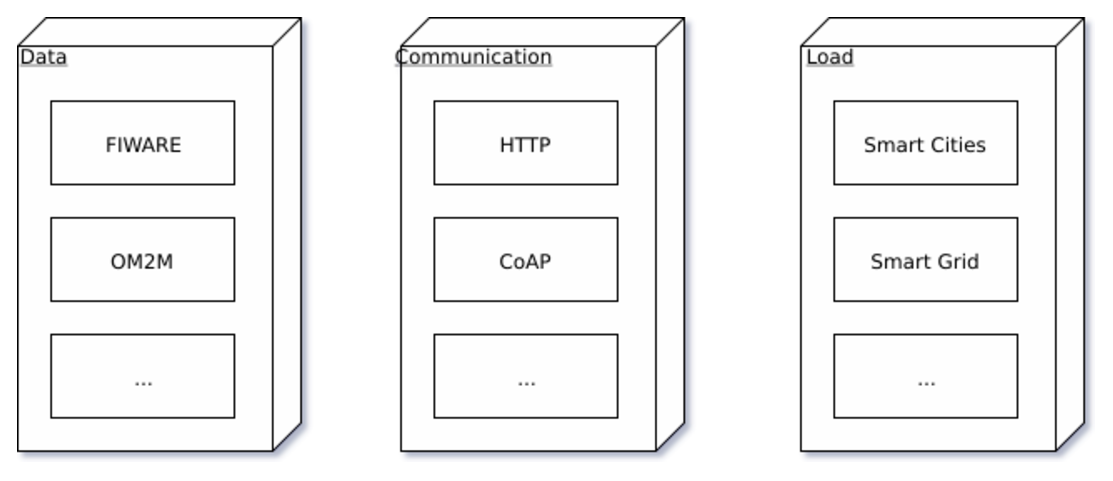
\includegraphics[width=\linewidth]{figures/benchmark_blocks.eps}
  \caption{Main architecture building blocks}
  \label{fig:main_building_blocks}
\end{figure}
%
\section{Evaluation}


\section{Conclusion}



% trigger a \newpage just before the given reference
% number - used to balance the columns on the last page
% adjust value as needed - may need to be readjusted if
% the document is modified later
%\IEEEtriggeratref{8}
% The "triggered" command can be changed if desired:
%\IEEEtriggercmd{\enlargethispage{-5in}}

% references section

% can use a bibliography generated by BibTeX as a .bbl file
% BibTeX documentation can be easily obtained at:
% http://mirror.ctan.org/biblio/bibtex/contrib/doc/
% The IEEEtran BibTeX style support page is at:
% http://www.michaelshell.org/tex/ieeetran/bibtex/
%\bibliographystyle{IEEEtran}
% argument is your BibTeX string definitions and bibliography database(s)
%\bibliography{IEEEabrv,../bib/paper}
%
% <OR> manually copy in the resultant .bbl file
% set second argument of \begin to the number of references
% (used to reserve space for the reference number labels box)

%\bibliographystyle{unsrt}
%\bibliography{biblio}


% that's all folks
\end{document}


%%% Local Variables:
%%% mode: latex
%%% TeX-master: t
%%% End:
=======
\documentclass{article}
\usepackage[utf8]{inputenc}
\begin{document}
(Type your content here.)
\end{document}
>>>>>>> f2e640db19cf7ec24c539f6c2c2fad5a3c77c44d
